\documentclass[11pt]{article}
\usepackage{fontspec}
\usepackage{caption}
\usepackage{polyglossia}
\usepackage{wrapfig}
\setdefaultlanguage{russian}
\setmainfont[Mapping=tex-text]{CMU Serif}
\usepackage{minted}
\newfontfamily{\cyrillicfonttt}[Scale=0.8]{Liberation Mono}
\usepackage[a4paper,includeheadfoot,margin=2.54cm]{geometry}

\title{CEL MeshWorks}
\author{Владимир Петриго}
\date{Ноябрь 2015}

\begin{document}

\maketitle

\section{Введение}

Стремительное развитие приобретает концепция Internet of Things (Интернет Вещей),
основной идеей которой является объединение различных устройств, датчиков, систем
управления и т.д. в единую сеть. В данной статье речь пойдет о платформе MeshWorks 
компании CEL, позволяющей организовать и настроить беспроводную ZigBee-сеть и организовать
к ней доступ из локальной или глобальной сети.

Для разработчиков доступны как готовые ZigBee-Ethernet- и ZigBee-USB-шлюзы, 
сенсорные узлы, так и отдельные модули, которые имеют встроенную 
прошивку-интерпретатор. Эта прошивка предоставляет возможность обработки скриптов, 
написанных на специальном скриптовом языке, похожем на язык Python, прямо на 
встроенном микроконтроллере. 
\section{Аппаратная платформа MeshWorks}

Компания CEL в своей линейке продукции, которая поддерживает работу с платформой 
MeshWorks, имеет как модули, так и готовые изделия.
% Module ZICM3588SP2 image
\begin{wrapfigure}{l}{0.3\textwidth}
  \begin{center}
    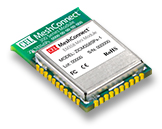
\includegraphics[width=0.25\textwidth]{mc_em358x_mini.jpg}
  \end{center}
  \caption{ZICM3588SP2}
\end{wrapfigure}
Модули ZICM3588SPx и ZICM357SPx построены на базе микросхем EM3588 и EM357 компании
Silicon Labs. Это системы на кристалле с микроконтроллерным ядром ARM Cortex-M3 и
встроенным ZigBee-приемопередатчиком, работающем на частоте 2.4 ГГц. Модули имеют
два исполнения - со встроенным усилителем мощности (максимальная выходная мощность
+20 дБм) и без него (максимальная выходная мощность +8 дБм). Благодаря высокой 
чувствительности встроенного приемопередатчика бюджет радиосвязи может достигать 
+123 дБ, что позволяет достичь дальности радиосвязи на открытых пространствах до 1 км,
а внутри помещений уверенно пробивать через бетонную стену. 

В таблице 1 представлены основные характеристики модулей ZICM3588SPx и ZICM357SPx[3].

\begin{table}[H]
    \begin{center}
    \caption{Характеристики модулей ZICM3588SPx и ZICM357SPx} 
    \begin{tabular}{|r|c|c|}
    \hline
    {} & \textbf{ZICM3588SPx} & \textbf{ZICM357SPx} \\
    \hline
    SoC & EM3588 & EM357 \\
    \hline
    GPIO & 23 & 19 \\
    \hline
    RAM & 64 Кб & 12 Кб \\
    \hline
    Flash & 512 Кб & 192 Кб \\
    \hline
    Мощность передатчика & \multicolumn{2}{c|}{+8/+20 дБм}\\
    \hline
    Чувствительность & \multicolumn{2}{c|}{-100/-103 дБм}\\
    \hline
    АЦП & \multicolumn{2}{c|}{5-канальный 14-разрядный}\\
    \hline
    Интерфейсы & \multicolumn{2}{c|}{SPI/I2C/UART}\\
    \hline
    USB & + & -\\
    \hline
    Температурный диапазон & \multicolumn{2}{c|}{-40..+85°С (-40..+125°С)}\\
    \hline
    Размеры & \multicolumn{2}{c|}{16 x 23 мм}\\
    \hline
    \end{tabular}
    \end{center}
\end{table}


Для возможности интегрировать ZigBee-сети с существующими серверными, настольными,
мобильными и прочими приложениями, компания CEL предлагает готовые ZigBee-USB- и 
ZigBee-Ethernet-шлюзы.

% USB and Ethernet Gateway images
\begin{wrapfigure}{l}{0.25\textwidth}
  \begin{center}
    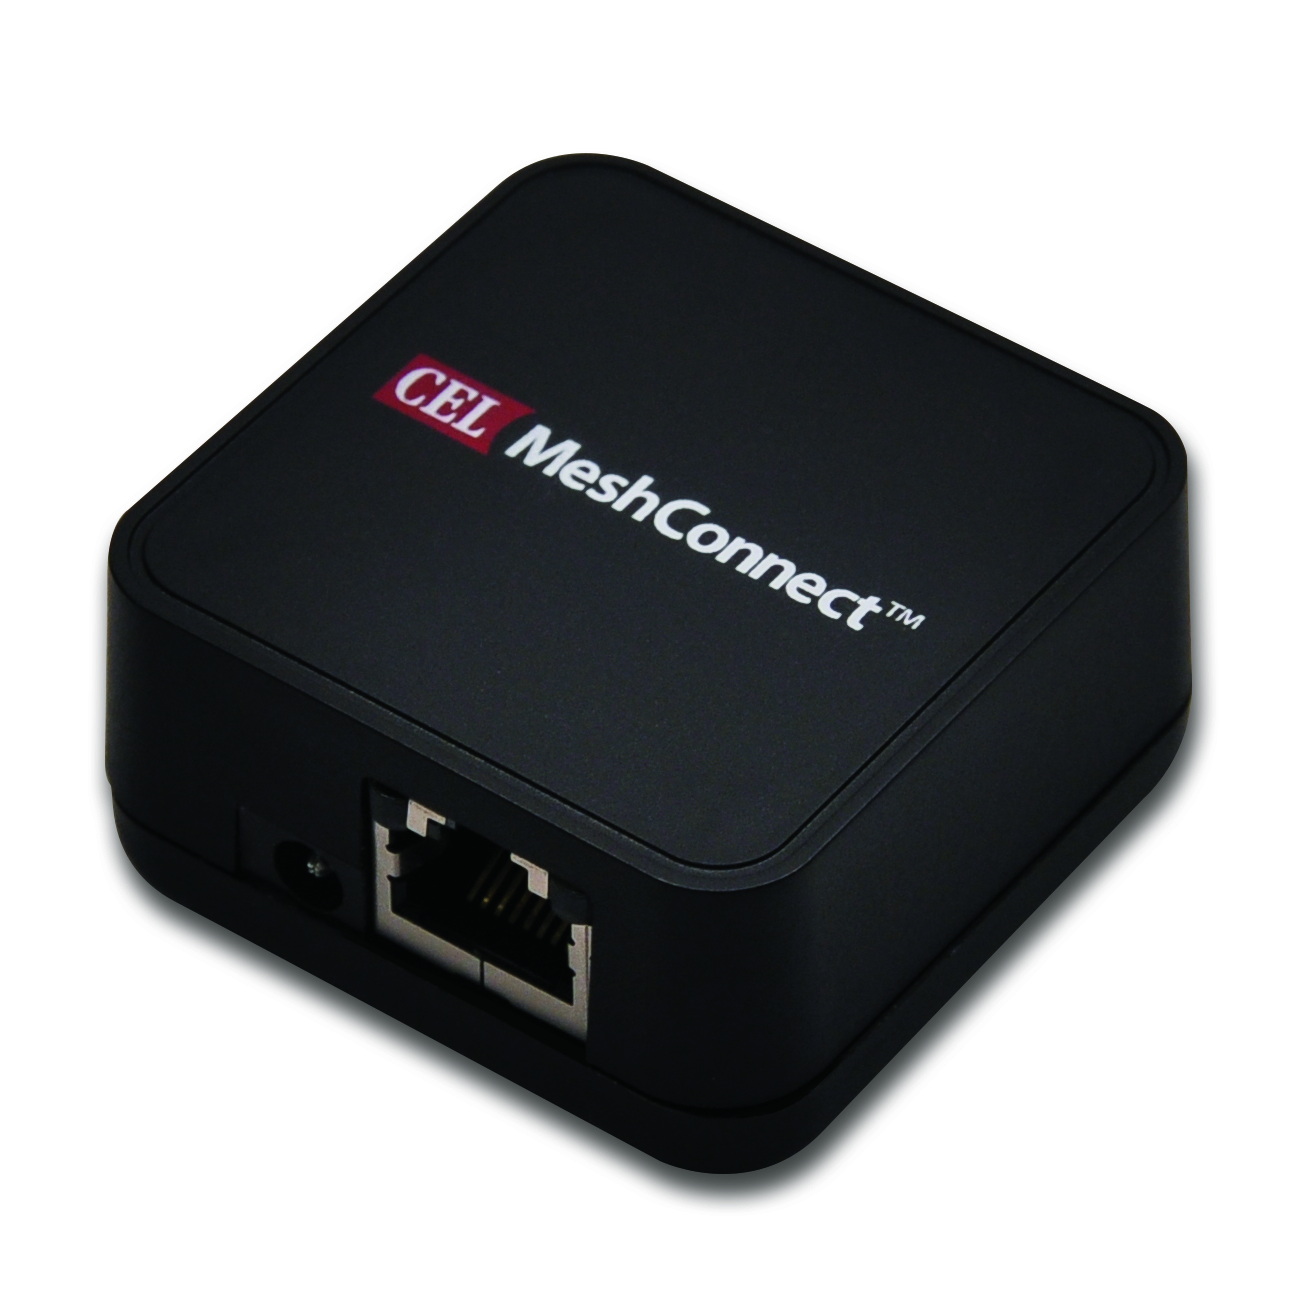
\includegraphics[width=0.20\textwidth]{gateway2.jpg}
  \end{center}
  \caption{ZMW-GW-ETH-1}
  \begin{center}
    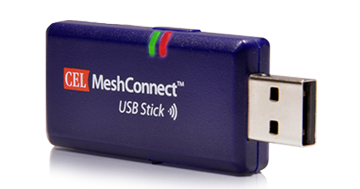
\includegraphics[width=0.20\textwidth]{usb_stick_em358_img_tech_plain.png}
  \end{center}
  \caption{ZM3588S-USB}
\end{wrapfigure}

Шлюзы ZMW-GW-ETH - это миниатюрные (5 х 5 х 2.5 см)[2] ZigBee-Ethernet-шлюзы, которые 
имеют встроенную прошивку MeshWorks и являются полноправными участниками
беспроводной сети. Эти шлюзы позволяют связать сеть MeshWorks с глобальной или 
локальной сетью. Все что нужно сделать, это добавить во встраиваемый в шлюз скрипт 
адрес внешнего сервера/приложения, если необходима отправка данных, и добавить
обработчик поступающих сообщений.

Пользователь может настроить поведение шлюза при поступлении информация от других 
узлов в сети MeshWorks (как будет сформировано сообщение, на какой адрес будет отправлено
и т.д.) с помощью специального интерфейса, предоставляемого скриптовым языком. 
Кроме этого, ZigBee-Ethernet-шлюзы могут обрабатывать входящие TCP/UDP/HTTP-сообщения.
Каждый шлюз настроен на получение IP-адреса по DHCP-интерфейсу и
внешнее приложение, зная его адрес, может совершать обмен данными через шлюз с любым
узлом сети MeshWorks.
\\\\
ZigBee-USB-шлюзы при подключении к компьютеру или другому устройству, распознается
как виртуальный COM-порт. Это позволяет добавить к существующим устройствам 
(например Wi-Fi-роутер с USB-разъемом, в которые можно загрузить собственное приложение;
персональный компьютер и т.д.) добавить возможность работы с сетями ZigBee. Шлюзы
как и модули имеют встроенную прошивку-интерпретатор, которая позволяет загружать
в них скрипты на языке MeshWorks. ZigBee-USB-шлюзы построены на базе модулей ZICM3588SPx и 
ZICM357SPx, поэтому все характеристики, приведенные в таблице 1, справедливы и для них.
\newpage
Кроме модулей и шлюзов для тестирования возможностей платформы MeshWorks и разработки
собственного набора предлагаются готовые сенсорные узлы OpenTether, имеющие в своем 
составе ряд датчиков и набор периферии:

\begin{minipage}{.6\textwidth}
  \begin{itemize}
    \item датчик влажности и температуры Si7013 (с интерфейсом I2C)
    \item акселерометр, гироскоп и компас MPU-9250 (с интерфейсом I2C)
    \item оптический бесконтактный датчик Si1143-M01 (с интерфейсом I2C)
    \item геркон
    \item 2 светодиода
    \item кнопка
    \item сирена
    \item разъем для подключения внешних устройств (аналоговых датчиков, I2C-устройств,
    цифровых входов/выходов)
  \end{itemize}
\end{minipage}
\begin{minipage}{.2\textwidth}
        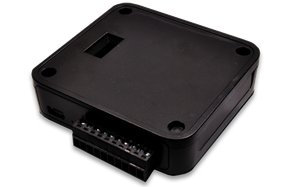
\includegraphics[width=1.2\textwidth]{sensor_node.png}
        \captionof{figure}{Сенсорный узел OpenTether}
\end{minipage}

Узлы ZMW-SENSOR-1 могут работать только в сетях, где остальные узлы также работают 
под управлением прошивки MeshWorks. Данный сенсорный узел дает возможность 
простого прототипирования и отладки собственного приложения.
Имеется несколько возможностей для питания сенсорного узла:
\begin{itemize}
 \item micro-USB-разъем
 \item 2xAAA батарейки
 \item DC-разъем (2.1 - 3.6 В)
\end{itemize}

По USB-интерфейсу осуществляется загрузка скрипта в подключенное устройство, либо 
его отправка на удаленный узел. Также по USB-интерфейсу осуществляется работа с
командным интерфейсом прошивки-интерпретатора, получение пользовательской и служебной
информации.

\section{Особенности платформы MeshWorks}

Как уже было упомянуто ранее, модули и шлюзы с поддержкой платформы MeshWorks имеют
встроенную прошивку, которая позволяет разработчику загружать в устройство Python-скриты.
Этот скрипт в реальном времени интерпретируется на конечном устройстве и это позволяет
задать общую логику работы.

Для того, чтобы начать работу с сетью MeshWorks требуется совершить несколько простых шагов:
\begin{enumerate}
    \item Необходимо выбрать координатор сети (устройство, которое создает сеть).
    \item Задать уникальное название сети MeshWorks
    \item Задать уникальные имена для каждого узла в сети.
    \item Выбрать, какие узлы могут переходить в спящий режим, а какие нет.
\end{enumerate}

Рассмотрим каждый шаг подробнее. Для того, чтобы определить устройство как координатор,
в загружаемом скриптовом файле необходимо инициализировать встроенную переменную 
\emph{celPy.DeviceName} строкой "Gateway"[1].

После этого необходимо указать строковое имя сети, которое с помощью специальных 
преобразований прошивкой-интерпретатором позволит однозначно идентифицировать сеть 
различным устройствам. Имя сети задается встроенной переменной \emph{celPy.ApplicationName}[1].
Имя сети может быть любым:
\begin{minted}[fontsize=\footnotesize]{python}
celPy.ApplicationName = "MeshWorks"
celPy.ApplicationName = "My Sensor Network"
\end{minted}

Для координатора данная переменная используется, чтобы создать сеть MeshWorks, к
которой смогут присоединяться беспроводные узлы, имеющие такое же имя сети в загруженном
скриптовом файле.

При присоединении к сети MeshWorks каждый узел имет собственный короткий 16-битовый
идентификатор. Так как скриптовый язык, используемый в платформе MeshWorks не поддерживает
непосредственную работу с короткими адресами[1], каждый узел должен иметь собственное
уникальное имя. Оно задается также, как и в случае с координатором, с помощью переменной
\emph{celPy.DeviceName}.

После всех этих шагов остался последний -- выбор типа устройства. Так как MeshWorks 
является надстройкой над стандартом ZigBee, то типы устройств унаследованы:
\begin{itemize}
    \item Координатор -- организатор сети.
    \item Роутер -- любое устройство, у которого встроенная переменная 
    \emph{celPy.IsSleepyDevice} имеет значение \textbf{False}. Через такие устройства
    осуществляется маршрутизация сообщений в сети.
    \item Спящее устройство -- любое устройство, у которого встроенная переменная 
    \emph{celPy.IsSleepyDevice} имеет значение \textbf{True}. Такие устройства уходят
    в спящий режим для экономии заряда сменного аккумулятора и через них не может
    осуществляться маршрутизация.
\end{itemize}

После выполнения всех рекомендаций устройства могут присоединяться к сети. Для того, чтобы
организовать передачу данных с удаленных узлов, необходимо понять, как платформа 
MeshWorks позволяет работать с периферией модулей.

Скриптовый язык поддерживает два объекта для работы с периферией ввода и вывода:

\begin{description}
    \item[Data Point (точка данных)] Используется для получения информации от 
    цифровых/аналоговых входов и от I2C-датчиков (I2C-датчики температуры, акселерометров,
    гироскопов, и т.д.)
    \item[Control Point (точка контроля)] Используется для выдачи управляющих цифровых 
    сигналов, работа с ШИМ, отправка данных на I2C-устройства вывода (дисплеи и т.д.)
\end{description}

\begin{figure}[h!]
    \centering
    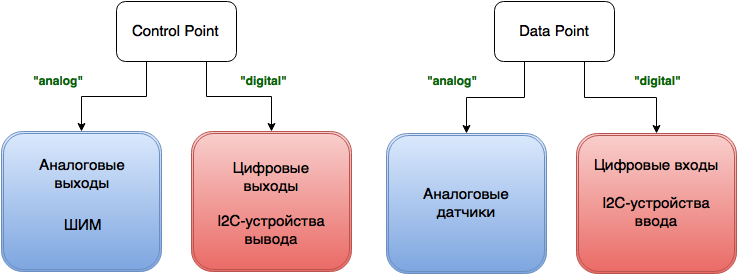
\includegraphics[scale=0.5]{DC_points.png}
    \caption{Структурная схема примера}
\end{figure}

Для того, чтобы создать любую точку необходимы две переменных[1]:

\begin{minted}[fontsize=\footnotesize]{python}
# variable = [<Имя точки>, GPIO, тип, callback-функция, время в секундах]
# values = [type, number, first value, second value]
\end{minted}

Callback-функция реализуется пользователем и будет автоматически вызываться через каждые
n-секунд (параметр «время в секундах»). Все необходимые точки контроля и точки данных
необходимо записать в специальные переменные \emph{celPy.DataCollectionPoints},
\emph{celPy.ControlPoints} и прошивка-интерпретатор сможет с ними работать.

После инициалицации точек данных и точек контрола в соответствующих им 
callback-функциях можно отправлять информацию на шлюз  о состоянии периферийного 
устройства (цифрового или аналогового) с помощью команды \emph{sendDataReport}.

\section{Пример работы}
В качестве примера, как работать с платформой MeshWorks, разберем простую задачу. 
Имеется две комнаты, температуру в которых необходимо измерить, а также есть два выключателя, 
которые должны управлять состоянием лампочек. И все данные о температуре и состоянии
выключателей должны передаваться на централизованный сервер. Примерная структурная
схема представлена на рисунке 1.
\begin{figure}[h!]
    \centering
    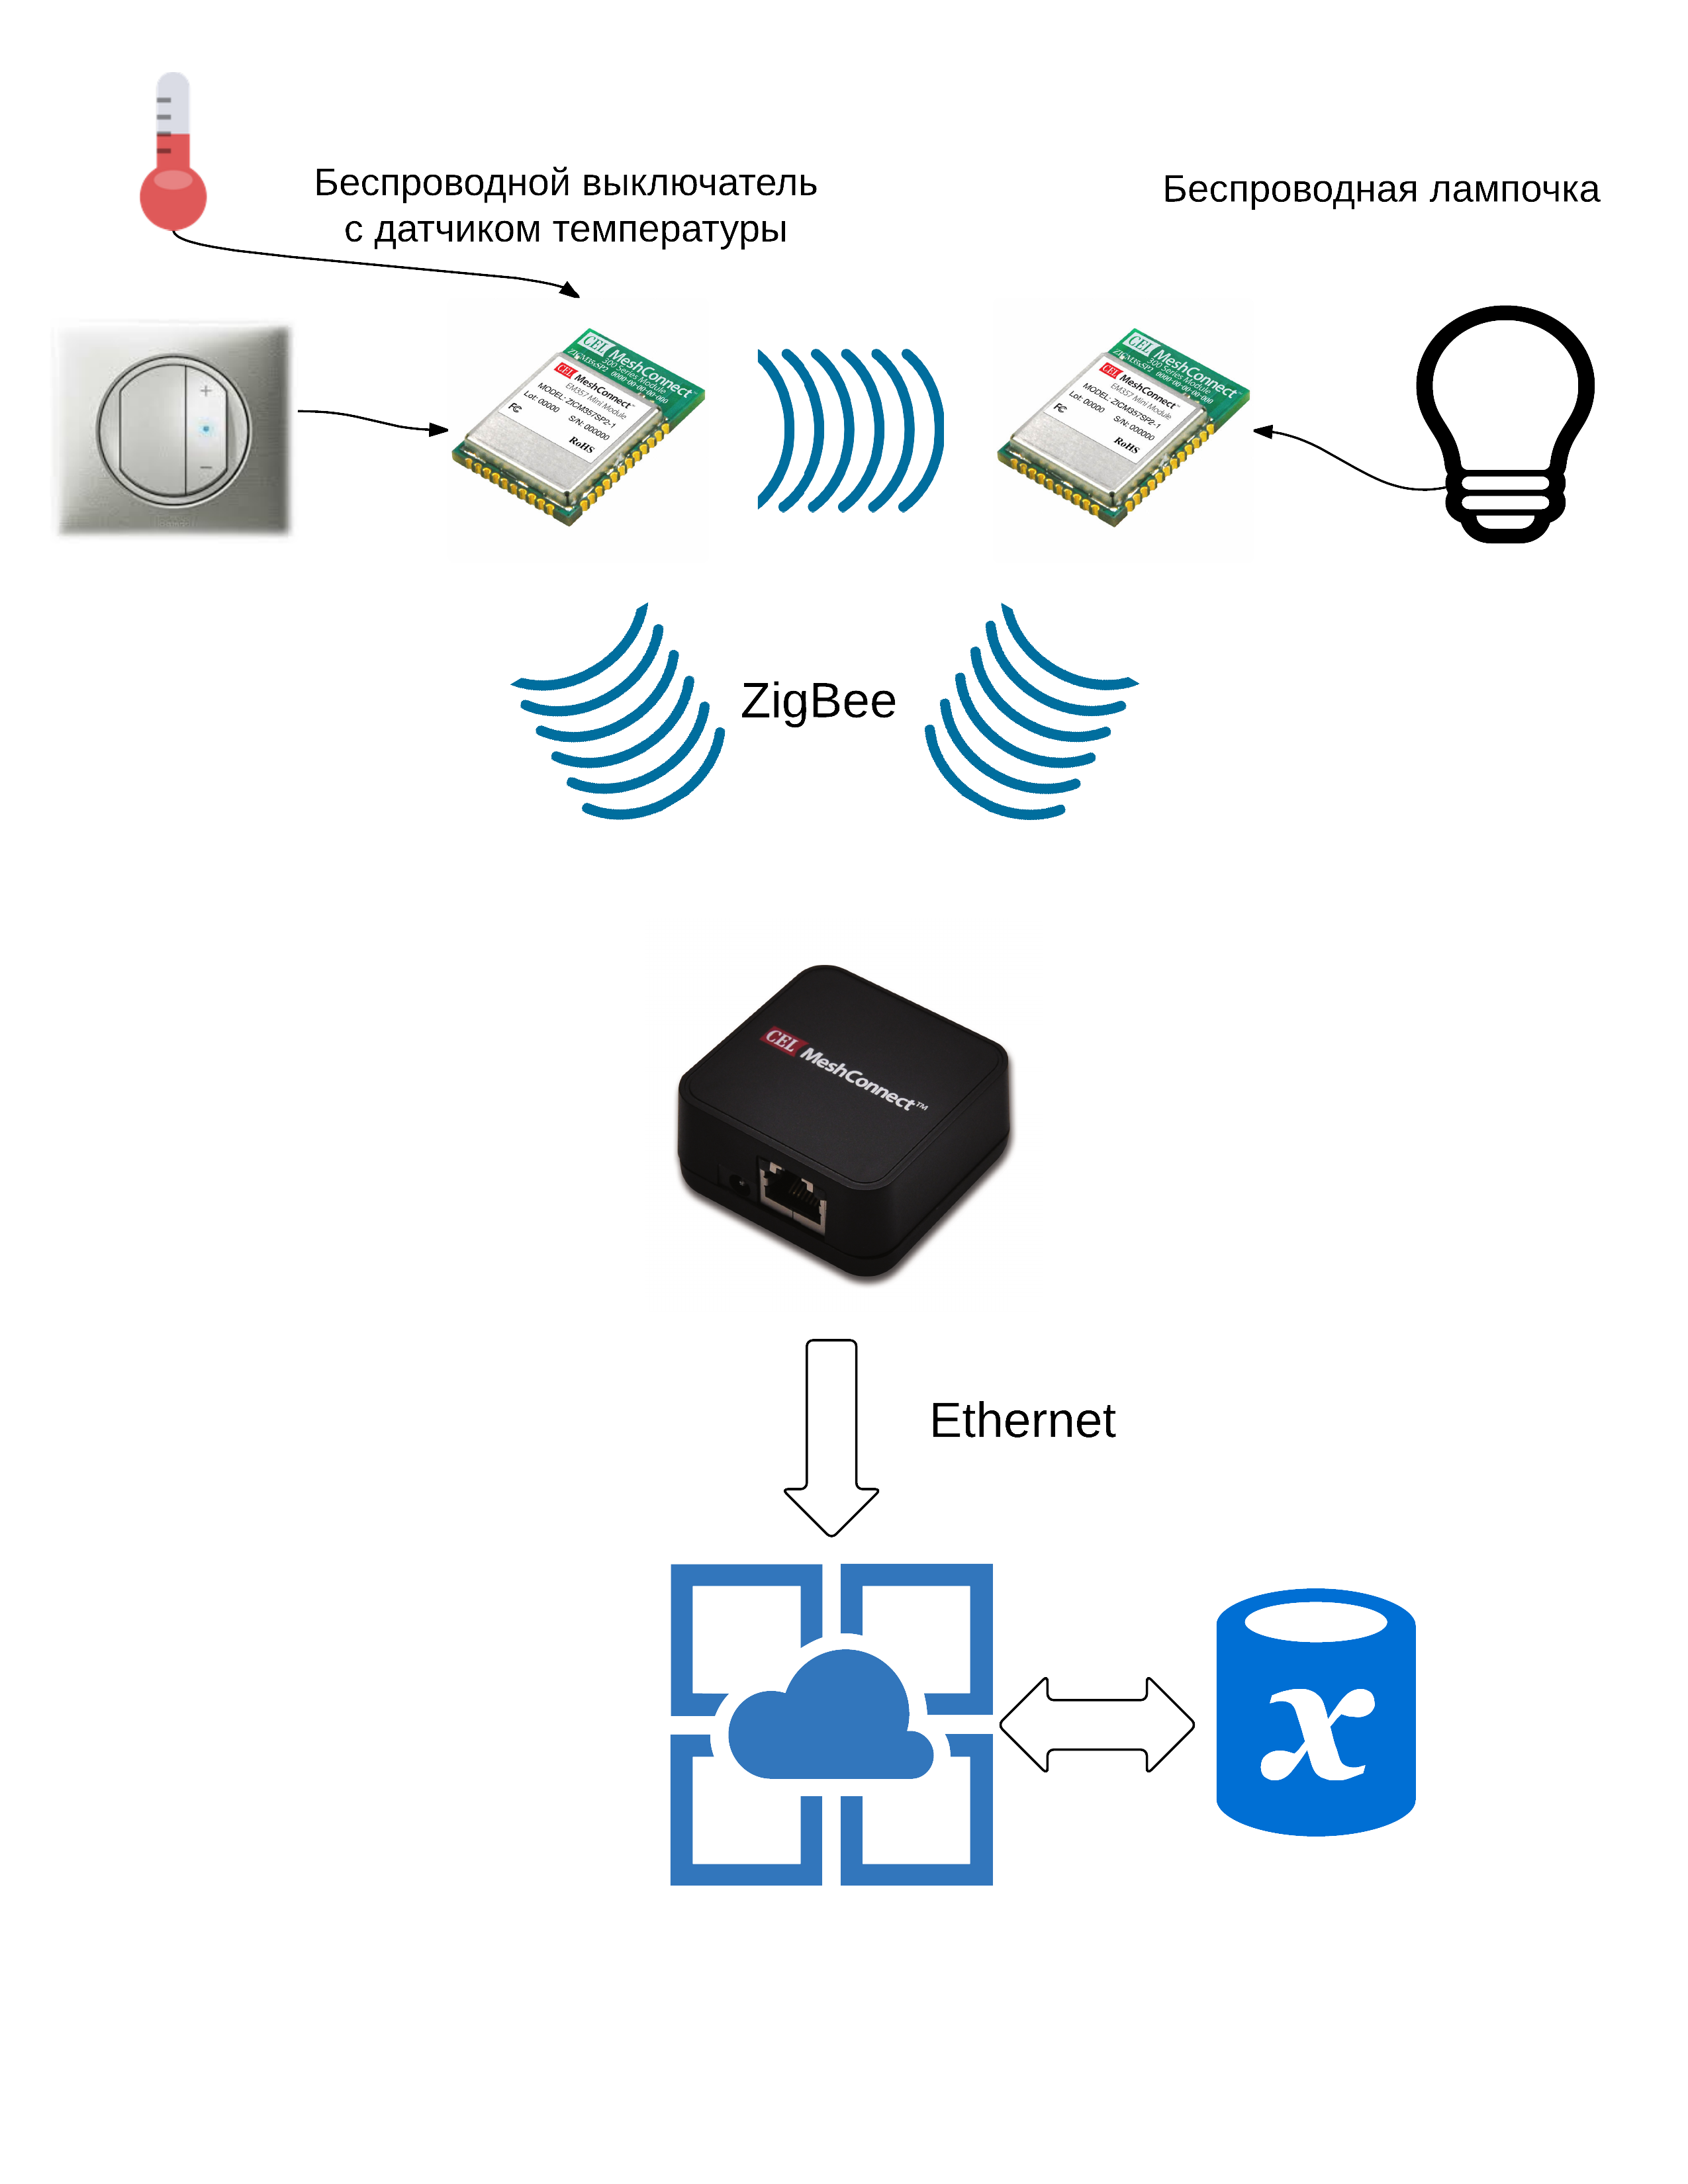
\includegraphics[scale=0.5]{cel-structure.png}
    \caption{Структурная схема примера}
\end{figure}

Выключатель, ламочка подключены к цифровым входам модуля CEL ZICM3588, в качестве
датчика температуры используется однокристальный датчик влажности и температуры
Si7013 с I2C-интерфейсом.

При изменении состояния выключателя лампочка включается или выключается. Также 1 раз в 20
секунд обновляется информация о значении температуры в комнате. Информацию об этом
каждый узел передает по радиоканалу на центральный шлюз. Центральный шлюз всю
полученную информацию передает на локальный или глобальный сервер.

Пример скрипта для узла сбора данных:
\begin{minted}[fontsize=\footnotesize]{python}
    # Светодиод на выводе PA6 
    greenLed = ["greenLed", "PA6", "digital", "grLedF", 1]
    greenValues = ["discrete", 2, "off", "on"]
    # Светодиод на выводе PA7 
    redLed = ["redLed", "PA7", "digital", "rdLedF", 1]
    redValues = ["discrete", 2, "off", "on"]
      
    # Data Point для кнопки
    button = ["button", "PB6", "digital", "buttonF", 1] 
    bValues = ["discrete", 2, "up", "down"] 
    
    prevButtonValue = 0
    buttonTickCount = 0 
      
    def buttonF():
        value = readDigital()
        # Периодическая отправка данных
        # о состоянии выключателя
        if (buttonTickCount > 30):
            buttonTickCount = 0
            sendDataReport(value, "button state")
        # если значение поменялось 
        if (value != prevButtonValue):  
            sendDataReport(value, "button state")
            # Устанавливаем состояние светодиода
            # в соответствии с состоянием выключателя
            celPy.AdjustLocalControlPoint("greenLed", value)    
        prevButtonValue = value
        buttonTickCount = (buttonTickCount + 1)
        
    # Data Point для датчика температуры
    tempSensor = ["tempSensor", "PA1", "i2c", "tempMeasFunc", 20]
    tempSensorValues = ["range", -40, 120]
    
    # Чтение температуры с Si7013
    def tempMeasFunc():
        value = readI2c(0x41, 0xE3, bigEndian)
        # Преобразование в градусы Цельсия
        value = (value * 175)
        value = (value / 65535)
        value = (value - 47)
        sendDataReport(value, "degrees C")
    
    celPy.addTickFunction(heartbeatLed, 20) 
      
    ledState = 0
      
    def heartbeatLed(): 
        if (ledState == 0): 
            celPy.AdjustLocalControlPoint("redLed", 1)
            ledState = 1
            return
        if (ledState == 1): 
            celPy.AdjustLocalControlPoint("redLed", 0)
            ledState = 0
      
    ####################################################
    # Сетевые настройки
    celPy.ApplicationName = "MeshWorks"  
    celPy.DeviceName = "Sensor 1" 
    celPy.IsSleepyDevice = False
    celPy.DataCollectionPoints = [button, tempSensor] 
    celPy.DataCollectionValues = [bValues, tempSensorValues]
    celPy.ControlPoints = [greenLed, redLed]
    celPy.ControlValues = [greenValues, redValues] 
      
    def main(): 
        pass
\end{minted}

Функциональность устройства определятся тремя основными функциями:
\begin{itemize}
    \item \emph{buttonF()} -- обрабатывает нажатие на кнопку (выключатель). При 
    изменении состояния светодиод (лампочка) переключается в соответствующее состояние.
    Об этом событии также отправляется сообщение на центральный шлюз. В приведенном
    выше примере также осуществляется отправка информации о текущем состоянии выключателя
    каждые 30 секунд.
    \item \emph{tempMeasFunc()} -- считывает данные с датчика
    Si7013 по интерфейсу I2C, переводит цифровые данные в градусы Цельсия и 
    отправляет эту информацию на центральный шлюз.
    \item \emph{heartbeatLed()} -- индикация работоспособности устройства. Переключает
    состояние вспомогательного красного светодиода каждые 2 секунды.
\end{itemize}

Пример скрипта для центрального Ethernet-шлюза:
\begin{minted}[fontsize=\footnotesize]{python}
# Конфигурация шлюза
celPy.ApplicationName = "MeshWorks"
celPy.DeviceName = "Gateway"
celPy.IsSleepyDevice = False

# Обработка сообщений от других сетевых устройств
def cpCallbackDataPointMessageReceived(deviceName, datapointName, discreteValueString, rangeValue):
    if (deviceName == "Sensor 1"):
        if (datapointName == "button"):
            udpPayload = deviceName
            udpPayload = (udpPayload + ": button=")
            udpPayload = (udpPayload + rangeValue)
            udp.send("192.168.22.225", 5555, udpPayload)
        if (datapointName == "tempSensor"): 
            udpPayload = deviceName
            udpPayload = (udpPayload + ": temp=")
            udpPayload = (udpPayload + rangeValue)
            udp.send("192.168.22.225", 5555, udpPayload) 
    if (deviceName == "Sensor 2"):
        if (datapointName == "button"):
            udpPayload = deviceName
            udpPayload = (udpPayload + ": button=")
            udpPayload = (udpPayload + rangeValue)
            udp.send("192.168.22.225", 5555, udpPayload)
        if (datapointName == "tempSensor"): 
            udpPayload = deviceName
            udpPayload = (udpPayload + ": temp=") 
            udpPayload = (udpPayload + rangeValue)
            udp.send("192.168.22.225", 5555, udpPayload)  
   
def main(): 
    pass

\end{minted}

Здесь функциональность определяется одной единственной функцией 
\emph{cpCallbackDataPointMessageReceived}, которая вызывается всякий раз, когда 
на шлюз поступает информация от других сетевых устройств. В зависимости от значения
переменной \emph{datapointName} (имя Data Point отправителя) и \emph{deviceName} (имя 
устройства) формируется соответствующее сообщение и отправляется на указанный адрес
сервера и порт.

После включения беспроводной сети и наличии доступа в локальную сеть, на сервер с адресом
\texttt{192.168.22.225:5555} начнут поступать UDP-сообщения вида:
\begin{minted}{bash}
    Sensor 1: temp=28
    Sensor 2: temp=19
    Sensor 2: button=1
\end{minted}
\newpage %% Put summary at the new page
\section{Заключение}
Платформа MeshWorks предлагает очень простой интерфейс для быстрой разработки систем
сбора данных, которые позволяют использовать практически все основные функциональные
особенности модулей ZICM3588SP2-1 на базе микросхем EM3588:
\begin{itemize}
 \item Работа с цифровыми портами ввода/вывода
 \item Подключение аналоговых датчиков
 \item Работа с устройствами и датчиками, использующими интерфейс I2C
 \item Поддержка спящих устройств, которые должны работать длительный срок от
 аккумуляторных или батарейных источников питания
\end{itemize}
Кроме этого компания CEL предоставляет устройства с Ethernet- и USB-интерфейсами, 
позволяющими расширить функциональность ZigBee-сетей, на базе платформы MeshWorks.
Это значительно упрощает интеграцию с серверными, настольными и мобильными приложениями.

\section{Список используемой литературы}

\begin{enumerate}
    \item MeshWorks™ Scripting Language User Guide / California Eastern Laboratories.--
    2015.- 29 стр.
    \item Ethernet Gateways / California Eastern Laboratories. -- 2015.– Режим доступа:
    \begin{verbatim}
    http://meshconnect.cel.com/docs/default-source/brochures/
    cel_ethernet_gateway_pb.pdf?sfvrsn=4}
    \end{verbatim}
    \item EM35x Mini Modules: ZICM35xSP0 and ZICM35xSP2 / California Eastern Laboratories. -- 2015.– Режим доступа:
    \begin{verbatim}
    http://meshconnect.cel.com/docs/default-source/data-sheets/
    em35x_mini_modules_ds.pdf?sfvrsn=17
    \end{verbatim}
\end{enumerate}
\end{document}
